\begin{frame}{parent and child processes}
\begin{itemize}
    \item every process (but process id 1) has a \textit{parent process} (\texttt{getppid()})
    \item this is the process that can wait for it
    \item creates tree of processes (Linux \texttt{pstree} command):
\end{itemize}
    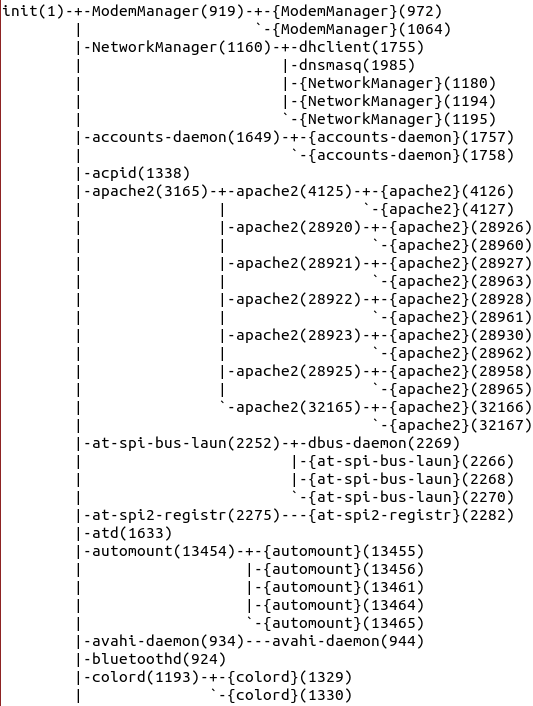
\includegraphics[height=0.6\textheight]{../unix-api/process-tree}
    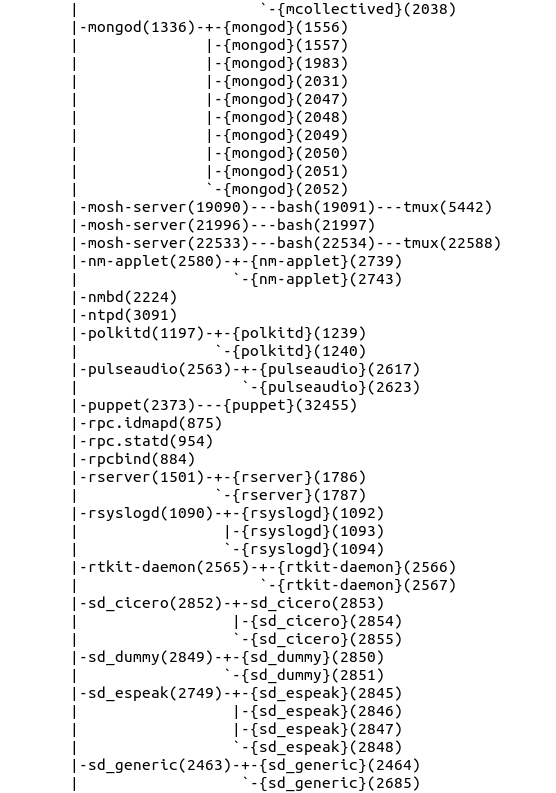
\includegraphics[height=0.6\textheight]{../unix-api/process-tree2}
\end{frame}

\begin{frame}{parent and child questions\ldots}
\begin{itemize}
    \item what if parent process exits before child?
        \begin{itemize}
        \item child's parent process becomes process id 1 (typically called \textit{init})
        \end{itemize}
    \item what if parent process never \texttt{waitpid()}s {\small (or equivalent)} for child?
        \begin{itemize}
        \item child process stays around as a ``zombie'' 
        \item can't reuse pid in case parent wants to use \texttt{waitpid()}
        \end{itemize}
    \item what if non-parent tries to \texttt{waitpid()} for child?
        \begin{itemize}
        \item waitpid fails
        \end{itemize}
\end{itemize}
\end{frame}
